%%%%%%%%%%%%%%%%%%%%%%%%%%%%%%%%%%%%%%%%%
%!TEX program = xelatex
%%%%%%%%%%%%%%%%%%%%%%%%%%%%%%%%%%%%%%%%%

%----------------------------------------------------------------------------------------
%	CLASS, PACKAGES AND OTHER DOCUMENT CONFIGURATIONS
%----------------------------------------------------------------------------------------

\documentclass[
	a4paper, % Paper size, use either a4paper or letterpaper
	%unnumberedsections, % Uncomment for no section numbering
]{ChaosEngineReport}


\newcommand{\signature}[3]{% <--- important %
    \vspace{15mm}
    Approved: \hrulefill
    
    \hspace*{0mm}\phantom{Approved: }\textbf{#1}
    
    \hspace*{0mm}\phantom{Approved: }#2 at #3
}
\usepackage{adjustbox}
\usepackage{graphicx}
\usepackage{tikz}
\usetikzlibrary{shapes.geometric, arrows.meta, positioning, fit,
                backgrounds, calc, decorations.pathreplacing}

\usepackage[table]{xcolor}
\usepackage{tabularx}
\usepackage{hyperref}
\usepackage[most]{tcolorbox}
\usepackage{pifont}
\usepackage{amssymb}
\newcommand{\cmark}{\ding{51}}
\newcommand{\xmark}{\ding{55}}
\newcommand{\diam}{\ensuremath{\blacklozenge}}
\tcbuselibrary{skins,breakable}
\newtcolorbox{callout_box}[2][]{breakable,sharp corners, skin=enhancedmiddle jigsaw,parbox=false,
boxrule=0mm,leftrule=2mm,boxsep=0mm,arc=0mm,outer arc=0mm,attach title to upper,
after title={\ }, coltitle=black,colback=gray!10,colframe=black, title={#2},
fonttitle=\bfseries,#1}
%--------------------------------------------------------------------------------------
%	REPORT INFORMATION
%----------------------------------------------------------------------------------------

\reporttitle{Asper London} % The report title to appear on the title page, include new lines if needed

\reportsubtitle{NFC Onboarding Proposal (DRAFT)} % Report subtitle, include new lines if needed

\reportauthors{Prepared for \textbf{Asper London} by:\\\smallskip Dr. Ahmed Al-Refaie (ahmed@chaos-engine.co) \\\smallskip Yassir Al-Refaie (yassir@chaos-engine.co)} % Report authors/group/department, include new lines if needed

\reportdate{\today} % Report date, include new lines for additional information if needed

\leftheadercontent{Asper London | NFC Onboarding} % Report title or other text to appear in the left header

\rightheadercontent{
\includegraphics[width=3cm]{logo-light-bg-v1.png}}

%----------------------------------------------------------------------------------------

% ── Colour palette ────────────────────────────────────────────────────────────
\usepackage[table]{xcolor}
\definecolor{Gold}{HTML}{B48C3C}
\definecolor{GoldLight}{HTML}{F7F0E0}
\definecolor{GoldMid}{HTML}{D4AA60}
\definecolor{Dark}{HTML}{1A1A2E}
\definecolor{Blue}{HTML}{1E4C8C}
\definecolor{BlueLight}{HTML}{EEF3FB}
\definecolor{Green}{HTML}{1A6B3C}
\definecolor{GreenLight}{HTML}{EAF7F0}
\definecolor{RowA}{HTML}{FFFFFF}
\definecolor{RowB}{HTML}{F8F8F8}
\definecolor{HeadBg}{HTML}{1A1A2E}
\definecolor{NoteGray}{HTML}{F4F4F4}
\definecolor{RuleGray}{HTML}{CCCCCC}
\definecolor{TextGray}{HTML}{555555}

% ── TikZ styles (reused throughout) ──────────────────────────────────────────
\tikzset{
  flowstart/.style={rectangle, rounded corners=7pt, minimum width=3.4cm,
    minimum height=0.72cm, text centered, draw=Gold, fill=Gold,
    text=white, font=\small\bfseries},
  flowproc/.style={rectangle, rounded corners=3pt, minimum width=3.8cm,
    minimum height=0.75cm, text centered, draw=Blue, fill=BlueLight,
    text=Dark, font=\small},
  flowdec/.style={diamond, minimum width=3.0cm, minimum height=0.85cm,
    aspect=2.3, text centered, draw=Gold, fill=GoldLight,
    text=Dark, font=\small},
  flowsys/.style={rectangle, rounded corners=3pt, minimum width=3.8cm,
    minimum height=0.75cm, text centered, draw=RuleGray, fill=NoteGray,
    text=Dark, font=\small},
  flowok/.style={rectangle, rounded corners=3pt, minimum width=3.8cm,
    minimum height=0.75cm, text centered, draw=Green, fill=GreenLight,
    text=Dark, font=\small},
  arr/.style={-{Stealth[length=5pt]}, thick, color=Dark},
  lbl/.style={font=\small, color=TextGray},
}

\begin{document}

%----------------------------------------------------------------------------------------
%	TITLE SECTION
%----------------------------------------------------------------------------------------

% The code here uses the information set in the REPORT INFORMATION block above and does not need to be modified unless you want to change the layout of the title section.

\thispagestyle{empty} % Suppress headers and footers on this page

\vspace*{-0.075\textheight} % Pull logo into top margin

\hfill
\includegraphics[width=5cm]{logo-light-bg-v1.png} % Right-aligned company logo

\vspace{0.06\textheight} % Vertical whitespace

{\large\raggedright\reportdate\par} % Report date

\vspace{0.01\textheight} % Vertical whitespace

{\fontsize{32pt}{34pt}\selectfont\raggedright\textbf{\reporttitle}\par} % Report title

\vspace{0.03\textheight} % Vertical whitespace

{\Large\raggedright\textit{\textbf{\reportsubtitle}}\par} % Subtitle

\vspace{0.06\textheight} % Vertical whitespace

{\large\raggedright\reportauthors\par} % Report authors, group or department

\vspace{0.12\textheight} % Vertical whitespace

%----------------------------------------------------------------------------------------



%----------------------------------------------------------------------------------------
%	TABLE OF CONTENTS
%----------------------------------------------------------------------------------------

\tableofcontents % Output the table of contents, automatically generated from the section commands used in the document

%----------------------------------------------------------------------------------------
%	SECTIONS AND PARAGRAPHS
%----------------------------------------------------------------------------------------
\newpage
\section{Executive Summary} 
This proposal outlines the technical approach, user flow, and implementation plan for the NFC device onboarding experience for embedded NFC chips in rings and wallet cards. The activation experience is designed to be frictionless and premium, consistent with a high-end product while remaining technically robust and scalable across multiple devices per user.

\begin{callout_box}{Scope Note:}
  The downstream functionality of the NFC chip - providing access to the wearer's medical records for first responders, family members, and carers - is out of scope for this document and is assumed to be handled by a separate, integrated system. Section~\ref{sec:url-routing} describes the URL routing behaviour that bridges the two systems.

  The User Interface is also assumed to be out-of-scope with the focus of this being on the backend and tooling required to achieve a satisfactory onboarding.
\end{callout_box}

\textbf{This document covers:}
\begin{itemize}
  \item NFC chip type selection and the implications for the onboarding flow
  \item End-to-end user onboarding flow, supporting both QR code and NFC tap methods
  \item URL routing behaviour post-activation (onboarding vs.\ medical profile)
  \item High-level implementation architecture and suggested technology stack
  \item Timeline and cost framework
  \item Security, accessibility, fulfilment, and regulatory considerations
  \item Open questions requiring stakeholder decision before detailed design begins
\end{itemize}

\section {Pre-requisite: NFC Chip Selection}

The choice of NFC chip is the single most consequential technical decision for this platform. It determines which activation methods are available, the level of security the platform can offer, and which future capabilities (e.g.\ dynamic content, tamper detection, provenance tracking) are possible without a chip change.
Chaos Engine is tasked with:

\subsection{Chip Comparison}

\begin{table}[h!]
\centering
\small
\rowcolors{2}{white}{gray!10}
\begin{tabularx}{\linewidth}{@{} L{3.2cm} X X X @{}}
  \toprule
  \textbf{Feature} & \textbf{NTAG213} & \textbf{NTAG424 DNA} & \textbf{MIFARE DESFire EV3} \\
  \midrule
  Standard & ISO 14443-A / Type 2 & ISO 14443-A / Type 4 & ISO 14443-A / Type 4 \\
  Static URL & \cmark{} Yes & \cmark{} Yes & \cmark{} Yes \\
  Dynamic/Signed URL & $\times$ No & \cmark{} SUN (Secure Unique NFC) & \cmark{} With custom app \\
  Clone protection & $\times$ None & \cmark{} Cryptographic SUN MAC & \cmark{} Mutual Auth (AES) \\
  iOS (no app required) & \cmark{} Native & \cmark{} Native & Limited --- may need app \\
  Android & \cmark{} Native & \cmark{} Native & \cmark{} Native \\
  Memory & 144 bytes & 416 bytes & 2--32 KB \\
  Typical unit cost & \textasciitilde£0.10 - 0.20 & \textasciitilde£0.40 - 0.70 & \textasciitilde£0.80 - 1.50 \\
  Complexity & Low & Medium & High \\
  \bottomrule
  Recommended & $\times$ & \textbf{\cmark{}\ Recommended} & \cmark{}\ If high security required \\
  \bottomrule
\end{tabularx}
\caption{NFC chip comparison for onboarding use case}
\end{table}

\newpage

\subsection{Recommendation: NTAG424 DNA}

The \textbf{NTAG424 DNA} is the recommended chip for this platform. Key reasons:

\begin{itemize}
  \item Supports native NFC scanning on iPhone (iOS~13+) and Android without requiring the user to install a dedicated app
  \item The \textbf{Secure Unique NFC (SUN)} feature generates a cryptographically signed, tap-unique URL on every interaction - embedding an encrypted counter and CMAC (Cipher-based Message Authentication Code)
  \item The backend can verify each scan is from a genuine chip without additional hardware, making cloning detectable
  \item The signed URL can carry both the device UID and a tap counter, enabling activation and subsequent medical record access from a single consistent tap
  \item Provides a foundation for future anti-counterfeiting or provenance features (e.g.\ resale authentication) without requiring a chip replacement
\end{itemize}

\begin{callout_box}{Future-proofing:}
If Aspers considers premium positioning around provenance verification or resale authentication, the NTAG424 DNA already provides the necessary cryptographic foundation. This makes it the right investment at this stage even if those features are not immediately planned.
\end{callout_box}

\subsection{Implications for the Onboarding Flow}

\begin{table}[h!]
\centering
\small
\rowcolors{2}{white}{gray!10}
\begin{tabularx}{\linewidth}{@{} X X @{}}
  \toprule
  \textbf{NTAG213 (Static URL)} &
  \textbf{NTAG424 DNA (SUN - Signed URL)} \\
  \midrule
   URL is fixed - identical on every tap & URL contains encrypted UID + incrementing tap counter \\
  No replay protection - chip cloning is undetectable & SUN MAC verified server-side - cloning is detectable \\
   Activation: URL-match against provisioned UID table & Activation: Cryptographic verification on first valid tap \\
  QR code and NFC tap flows are architecturally identical & NFC tap carries verifiable context QR cannot replicate \\
   Lower chip cost (\textasciitilde£0.10 - 0.20) & Moderate chip cost (\textasciitilde£0.40 - 0.70) \\
\end{tabularx}
\caption{Flow implications by chip type}
\end{table}

\newpage

\section{URL Routing - Activation vs.\ Medical Profile}
\label{sec:url-routing}

As part of the flow, the same url encoded on the chip has to serve two functions
\begin{enumerate}
\item It has to register the device to a user and activate it;
\item thereafter, it has to lead the scanner to the users medical profile
\end{enumerate}

This is handled through the backend, with \textbf{the URL on the chip never changing}. The backend works as a router that decides how to proceed based on the curent device ID (UID) from the URL.

\begin{center}
  \begin{adjustbox}{width=\linewidth} % This forces it to the margins
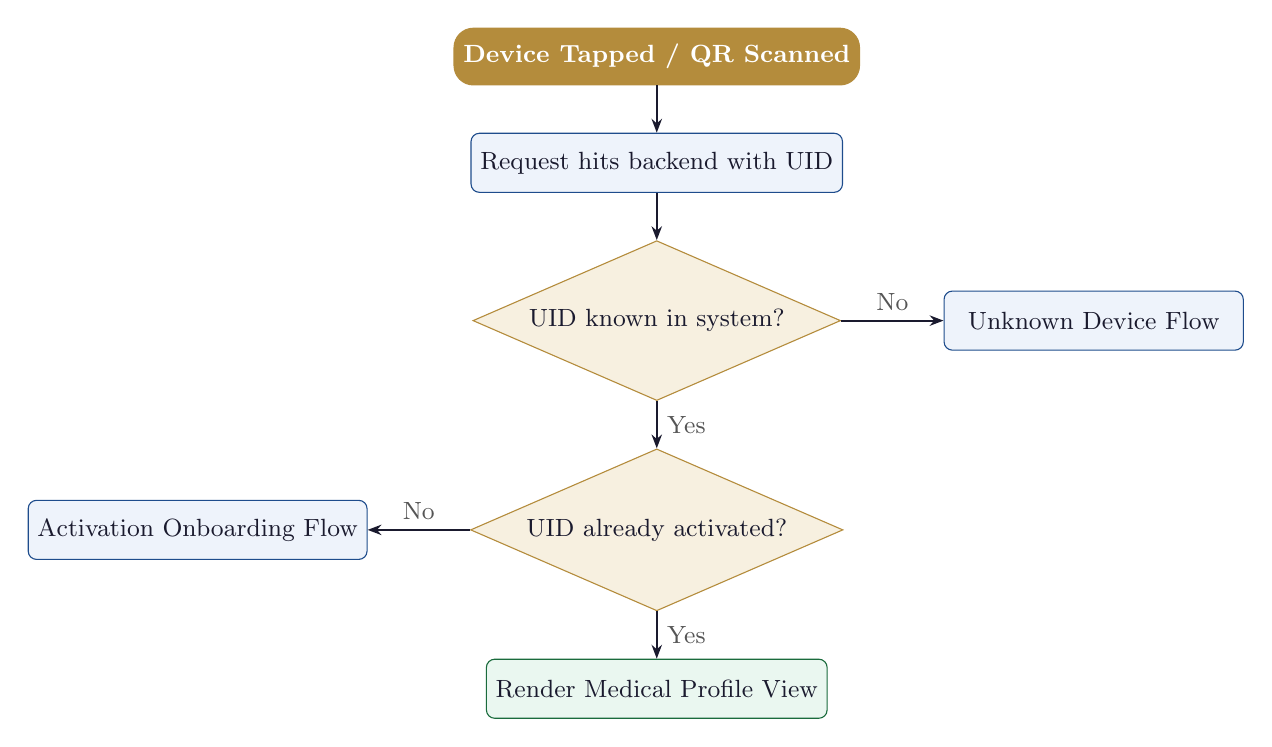
\begin{tikzpicture}[node distance=0.6cm and 1.2cm]
  \node (tap)   [flowstart]                          {Device Tapped / QR Scanned};
  \node (req)   [flowproc, below=of tap]             {Request hits backend with UID};
  \node (known) [flowdec,  below=of req]             {UID known in system?};
  \node (err)   [flowproc, right=1.3cm of known]     {Unknown Device Flow};
  \node (actd)  [flowdec,  below=of known]           {UID already activated?};
  \node (onb)   [flowproc, left=1.3cm of actd]       {Activation Onboarding Flow};
  \node (med)   [flowok,   below=of actd]            {Render Medical Profile View};

  \draw[arr] (tap)   -- (req);
  \draw[arr] (req)   -- (known);
  \draw[arr] (known) -- node[above, lbl]{No}  (err);
  \draw[arr] (known) -- node[right, lbl]{Yes} (actd);
  \draw[arr] (actd)  -- node[above, lbl]{No}  (onb);
  \draw[arr] (actd)  -- node[right, lbl]{Yes} (med);
\end{tikzpicture}
\end{adjustbox}
\end{center}

\vspace{4pt}
In practice, the single endpoint \texttt{https://id.brand.com?uid=XXXX} (or with SUN parameters for NTAG424) behaves as follows:

\begin{enumerate}
  \item \textbf{First tap - unactivated:} Backend finds the UID in the provisioned-but-unclaimed table. Renders the onboarding and account creation flow.
  \item \textbf{Subsequent taps - activated:} Backend finds the UID bound to a user profile. Redirects to the medical profile view, subject to whatever access control policy has been configured.
  \item \textbf{Unknown UID:} May indicate a fulfilment error or counterfeit device. Surfaces a support contact with the UID shown for reference.
\end{enumerate}

\newpage

\subsection{Access Control on the Medical Profile View}

Because the same tap that was used for onboarding will later be used by first responders, family members, or carers, the access model for the medical profile view is a product decision with real safety implications. Three approaches exist:

\begin{table}[h!]
\centering
\small
\rowcolors{2}{white}{gray!10}
\begin{tabularx}{\linewidth}{@{} L{2.8cm} X L{3.0cm} @{}}
  \toprule
  \textbf{Model} &
  \textbf{Behaviour} &
  \textbf{Trade-off} \\
  \midrule
  \textbf{Open / No auth} & Tap immediately shows the medical profile. No login required. & Best for emergencies; anyone who holds the ring can view it. \\
  \textbf{PIN or access code} & A short PIN (printed on a companion card in the wearer's wallet) is entered by the responder before the profile is shown. & Adds a layer of protection; adds friction in time-critical situations. \\
  \textbf{Tiered access} & Unauthenticated tap shows only critical info (blood type, allergies, emergency contact). Full records require an authenticated session. & Balances safety and privacy; recommended approach for most deployments. \\
\end{tabularx}
\caption{Medical profile access control models}
\end{table}

\begin{callout_box}{Recommendation:}
The tiered model is the most robust default. Critical data (blood type, known allergies, emergency contact number) should be immediately visible on any tap - because a first responder cannot be expected to have an account. Full medical records can sit behind authentication for family members and carers who have a pre-existing relationship with the platform. This decision should be made explicit before the medical profile system is scoped.
\end{callout_box}

\newpage

\section{Onboarding Flow}
The onboarding flow is designed with two entry points, QR code scan and NFC tap, that converge into a single unified registration journey. The experience is intentionally minimal, mirroring the approach taken by services like Monzo's card activation.

This authenticating user's ID would be encoded via URL parameter (https://id.brand.ltd?device=XX231\textbf{?user=uudd88221}) to identify who is trying to register the device to their account.

\newpage

\subsection{Flow Diagram}

\begin{figure}[h!]
  \centering
  \begin{adjustbox}{width=\linewidth} % This forces it to the margins
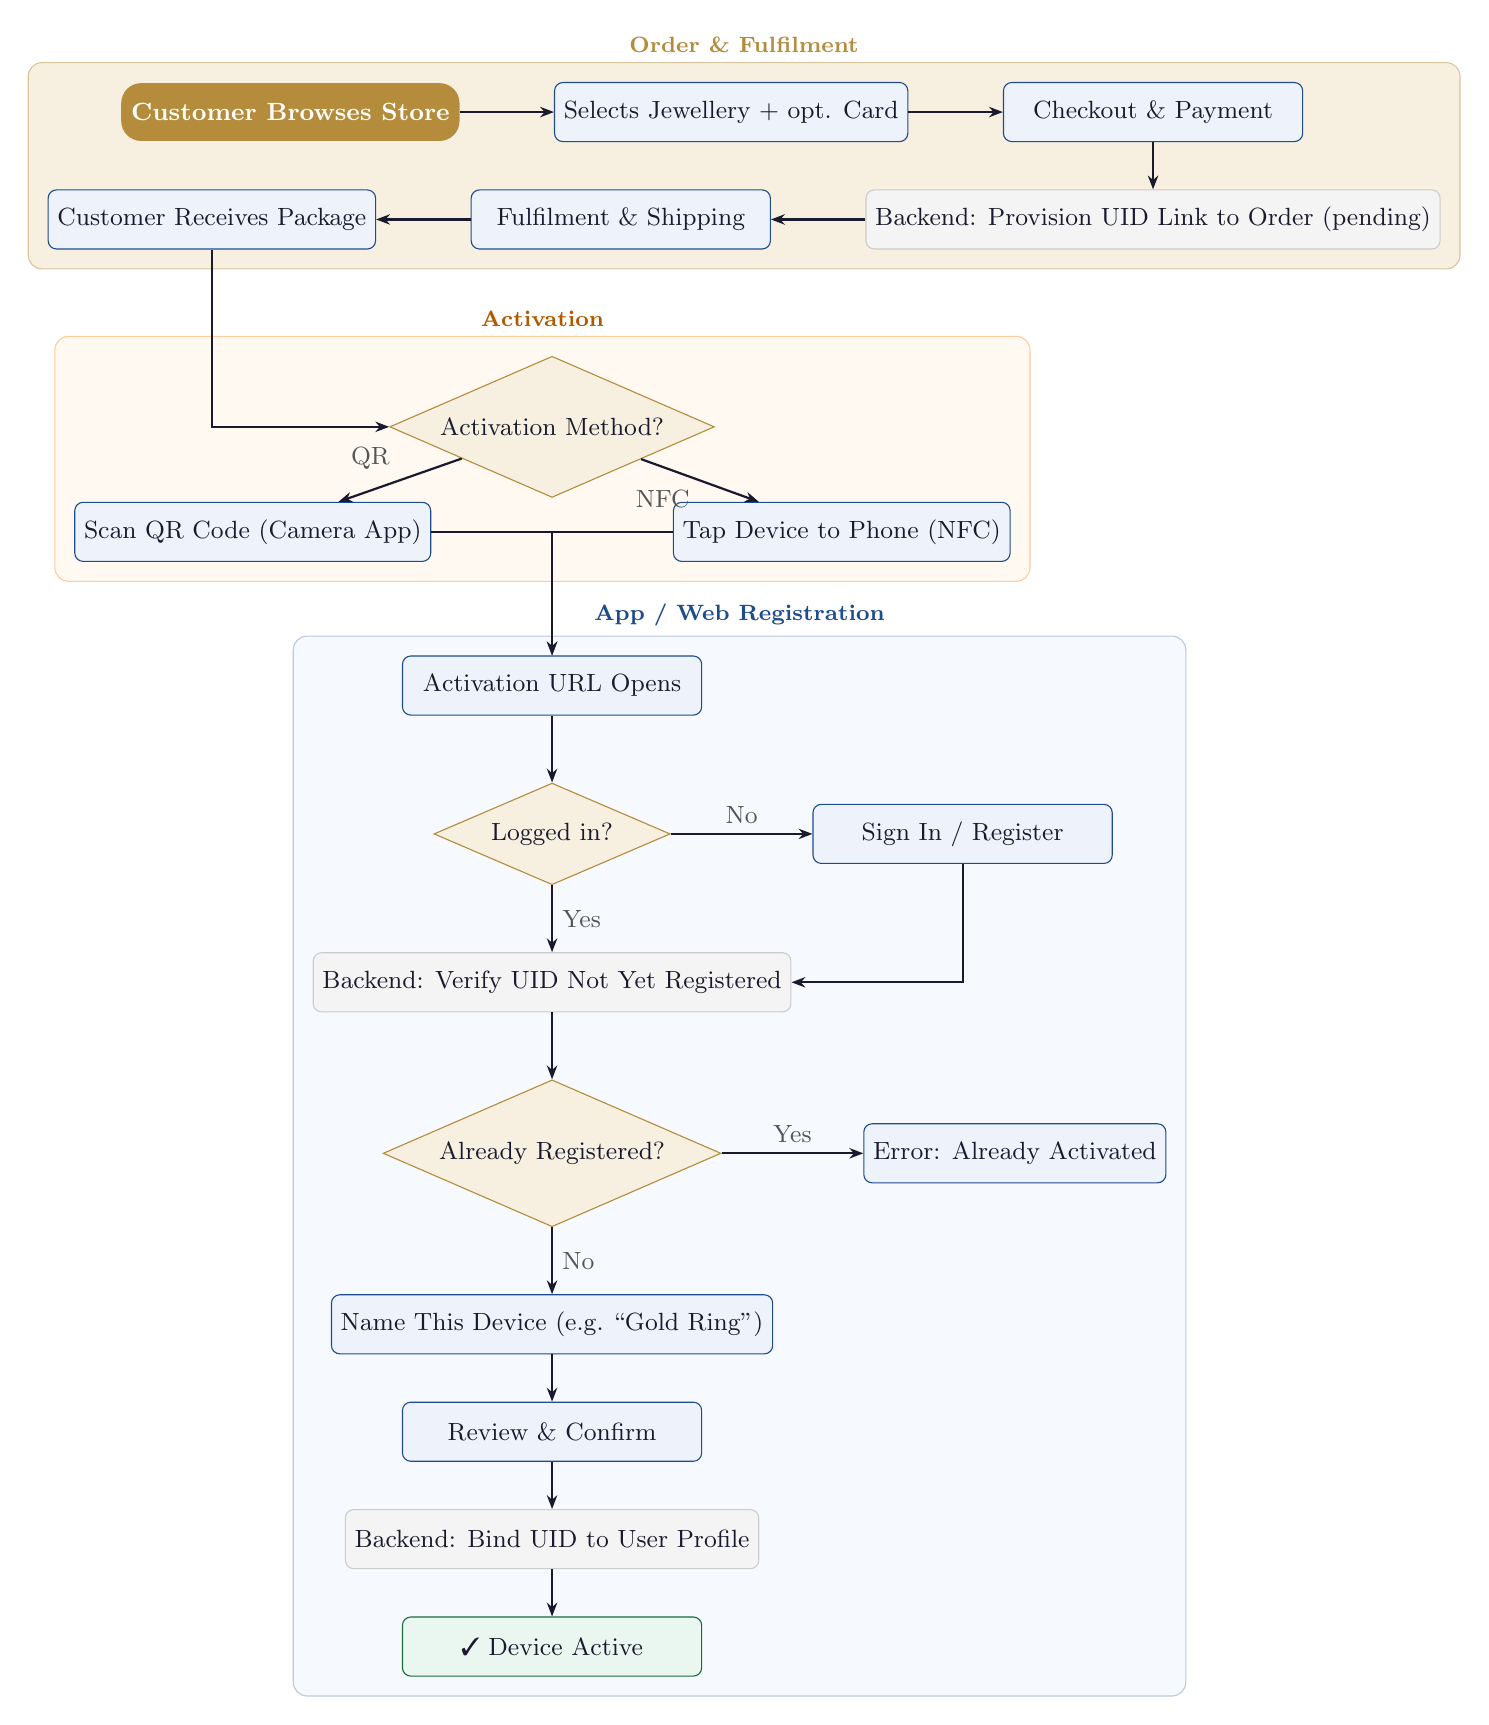
\begin{tikzpicture}[node distance=0.6cm and 1.2cm]

  %% ── Col 1: Order & Fulfilment ────────────────────────────────────────────
  \node (start)   [flowstart]                             {Customer Browses Store};
  \node (order)   [flowproc, right=of start]              {Selects Jewellery + opt. Card};
  \node (pay)     [flowproc, right=of order]              {Checkout \& Payment};
  \node (fulfil)  [flowsys,  below=of pay]                {Backend: Provision UID Link to Order (pending)};
  \node (ship)    [flowproc, left=of fulfil]             {Fulfilment \& Shipping};
  \node (recv)    [flowproc, left=of ship]               {Customer Receives Package};

  %% ── Col 2: Activation ────────────────────────────────────────────────────
  \node (choice)  [flowdec,  below right=1.8cm and 1.2cm of recv]         {Activation Method?};
  \node (qr)      [flowproc, below left=0.5cm and 0.5cm of choice] {Scan QR Code (Camera App)};
  \node (nfc)     [flowproc, below right=0.5cm and 0.5cm of choice] {Tap Device to Phone (NFC)};

  %% ── Col 3: App / Web ─────────────────────────────────────────────────────
  \node (land)    [flowproc, below=2cm of choice]       {Activation URL Opens};
  \node (authq)   [flowdec,  below=0.85cm of land]        {Logged in?};
  \node (login)   [flowproc, right=1.8cm of authq]        {Sign In / Register};
  \node (verify)  [flowsys,  below=0.85cm of authq]       {Backend: Verify UID Not Yet Registered};
  \node (regq)    [flowdec,  below=0.85cm of verify]      {Already Registered?};
  \node (errdup)  [flowproc, right=1.8cm of regq]         {Error: Already Activated};
  \node (name)    [flowproc, below=0.85cm of regq]        {Name This Device (e.g.\ ``Gold Ring'')};
  \node (confirm) [flowproc, below=of name]               {Review \& Confirm};
  \node (backend) [flowsys,  below=of confirm]            {Backend: Bind UID to User Profile};
  \node (done)    [flowok,   below=of backend]            {\cmark{}\ Device Active};

  %% ── Arrows: col 1 ────────────────────────────────────────────────────────
  \draw[arr] (start)   -- (order);
  \draw[arr] (order)   -- (pay);
  \draw[arr] (pay)     -- (fulfil);
  \draw[arr] (fulfil)  -- (ship);
  \draw[arr] (ship)    -- (recv);
  \draw[arr] (recv)    |- (choice);

  %% ── Arrows: choice ───────────────────────────────────────────────────────
  \draw[arr] (choice) -- node[above left, lbl]{QR}  (qr);
  \draw[arr] (choice) -- node[below left, lbl]{NFC} (nfc);
  \draw[arr] (qr)  -| (land);
  \draw[arr] (nfc) -| (land);

  %% ── Arrows: col 3 ────────────────────────────────────────────────────────
  \draw[arr] (land)    -- (authq);
  \draw[arr] (authq)   -- node[right, lbl]{Yes} (verify);
  \draw[arr] (authq)   -- node[above, lbl]{No}  (login);
  \draw[arr] (login)   |- (verify);
  \draw[arr] (verify)  -- (regq);
  \draw[arr] (regq)    -- node[right, lbl]{No}  (name);
  \draw[arr] (regq)    -- node[above, lbl]{Yes} (errdup);
  \draw[arr] (name)    -- (confirm);
  \draw[arr] (confirm) -- (backend);
  \draw[arr] (backend) -- (done);

  %% ── Lane backgrounds ─────────────────────────────────────────────────────
  \begin{scope}[on background layer]
    \node[fill=GoldLight, draw=Gold!50, rounded corners=5pt,
      fit=(start)(recv)(order)(pay)(fulfil)(ship), inner sep=7pt,
      label={[font=\footnotesize\bfseries, color=Gold]above:Order \& Fulfilment}] {};
    \node[fill=orange!5, draw=orange!40, rounded corners=5pt,
      fit=(choice)(qr)(nfc), inner sep=7pt,
      label={[font=\footnotesize\bfseries, color=orange!70!black]above:Activation}] {};
    \node[fill=BlueLight!50, draw=Blue!30, rounded corners=5pt,
      fit=(land)(done)(login)(errdup)(authq)(verify)(regq)(confirm)(backend), inner sep=7pt,
      label={[font=\footnotesize\bfseries, color=Blue]above:App / Web Registration}] {};
  \end{scope}
\end{tikzpicture}
\end{adjustbox}
\caption{End-to-end NFC device onboarding flow}
\end{figure}

\newpage

\subsection{Phase 1 - Order \& Fulfilment}

The customer browses the store and selects a jewellery piece. At checkout, they may optionally add a wallet card to their order. Upon payment confirmation, the backend provisionally assigns the NFC chip UID (pre-encoded at the factory or at fulfilment) to a \textit{pending} status. At this stage the device is expecting a user in the system but not yet bound or activated - it cannot provide access to any medical profile until the customer completes the activation step.

The fulfilment pack should include:
\begin{itemize}
  \item The jewellery item with embedded NFC chip
  \item Optional: NFC wallet card
  \item A card or booklet with the QR code and brief activation instructions
  \item A printed short URL as a typed fallback for devices without NFC reader access
\end{itemize}

\subsection{Phase 2 - Activation Method}

When the customer receives their order, they initiate activation via one of two methods:

\begin{table}[h!]
\centering
\small
\rowcolors{2}{white}{gray!10}
\begin{tabularx}{\linewidth}{@{} X X @{}}
  \toprule
  \textbf{Method A - QR Code Scan} &
  \textbf{Method B - NFC Tap} \\
  \midrule
  Customer opens their phone camera and scans the QR code printed in the packaging. This opens the activation URL in the browser. &
  Customer holds the NFC chip (ring or card) near the top of their phone. The phone reads the chip and opens the activation URL automatically. \\

  Recommended for: users unfamiliar with NFC, older devices, or as a fallback. &
  Primary method for most smartphones (iOS~13+ and Android). \\

  QR encodes a static URL with the UID as a query parameter. &
  NFC URL includes a cryptographic SUN signature for NTAG424; or a static UID URL for NTAG213. \\
\end{tabularx}
\caption{Activation method comparison}
\end{table}

\subsection{Phase 3 - App / Web Registration}

Both methods resolve to the same activation web application. The steps from this point are:

\begin{enumerate}
  \item \textbf{Authentication check}: if the user is already signed in, they proceed directly. If not, they are prompted to sign in or create an account. A magic link (passwordless email) or OAuth (Google/Apple Sign-In) is strongly recommended to minimise friction on mobile.

  \item \textbf{UID verification}: the backend checks whether the UID is known (provisioned at fulfilment) and has not yet been registered to any account. If the UID is already registered, the user sees an ``already activated'' message with options to contact support.

  \item \textbf{Device naming}: the user is invited to give the device a friendly name (e.g.\ ``Gold Ring'', ``Wallet Card''). For users registering multiple devices, this is essential for distinguishing them in the profile dashboard.

  \item \textbf{Confirmation \& binding}: the user reviews a summary and confirms. The backend atomically binds the UID to the user's profile, marks the device as active, and sends a confirmation email.

  \item \textbf{Success screen}: a confirmation is shown. The user is invited to continue to their profile to set up their medical information (handled by the out-of-scope medical records system).
\end{enumerate}

Activation can either be through a web login via the URL, or if the customer is in the app, they can avoid the login by using a guided flow on the phone that will ask them to Scan the QR or NFC chip at a specific point in the process, much like the Monzo card activation.

\subsection{Multi-Device Registration}

Users who purchase multiple items can register all devices to the same profile. Each device has its own UID and is activated independently using either the QR or NFC method. From the profile dashboard, users can see all registered devices, rename them, deactivate them individually, or transfer them.

\subsection{Edge Cases \& Error Handling}

\begin{table}[h!]
\centering
\small
\rowcolors{2}{white}{gray!10}
\begin{tabularx}{\linewidth}{@{} L{3.8cm} X @{}}
  \toprule
  \textbf{Scenario} &
  \textbf{Handling} \\
  \midrule
  Device already activated & Show friendly error. Offer contact support option, or initiate a device transfer flow. \\
  UID not found in system & May indicate a fulfilment error or counterfeit chip. Surface a support prompt with the UID displayed for reference. \\
  NFC not supported on device & QR code fallback is always available in-box. The web app detects NFC capability and guides accordingly. \\
  User loses account access & Standard account recovery (email verification). UID remains bound until explicitly deactivated by support. \\
  Lost or stolen device & User can freeze (temporary) or deactivate (permanent) individual devices from the dashboard without affecting others. This is a simple flag in the backend that is changed based on user input \\
  SUN MAC verification failure (NTAG424) & Log the event, surface a support prompt. May indicate a tampered or cloned chip. \\
  Tap counter regression (NTAG424) & Flag as potential replay attack. Block activation, log event, alert ops. \\
\end{tabularx}
\caption{Edge cases and error handling}
\end{table}

\newpage

\section{High-Level Implementation}

\subsection{System Architecture}

The platform comprises four main components:

\begin{table}[h!]
\centering
\small
\rowcolors{2}{white}{gray!10}
\begin{tabularx}{\linewidth}{@{} L{3.0cm} X @{}}
  \toprule
  \textbf{Component} &
  \textbf{Description} \\
  \midrule
  NFC Chips & NTAG424 DNA chips pre-encoded with the activation URL template and SUN configuration. Encoded and tested during manufacturing or fulfilment. \\
  Web and/or Native App & Serving the activation and post-activation routing logic. Works in-browser with no install required. \\
  Backend API & UID provisioning, SUN MAC verification, authentication, device registration, profile management, and webhook triggers for the medical records system. \\
  Admin / Ops Dashboard & Internal tool for: batch UID provisioning, fulfilment status tracking, support tooling (manual deactivation, device transfer), and audit log access. \\
\end{tabularx}
\caption{Platform components}
\end{table}

\subsection{NFC Chip Provisioning}

Each chip UID must be registered in the backend before it leaves the warehouse:

\begin{itemize}
  \item Chips are encoded with the activation URL at the factory or fulfilment centre using an NXP-compatible programming station
  \item For NTAG424: SUN is configured with a brand-specific AES-128 key pair. The key is stored in the backend secrets manager (AWS Secrets Manager or HashiCorp Vault) - never in application code
  \item Each UID is written to the backend database with status \texttt{provisioned} (linked to the corresponding order ID after dispatch?)
  \item QR codes are generated server-side from the same UID and printed on the activation insert card, automatable as part of the order fulfilment pipeline
\end{itemize}

\subsection{Authentication}

To keep the activation flow frictionless for a consumer audience, the recommended approach is:

\begin{itemize}
  \item \textbf{Magic link} (passwordless email) as the primary method
  \item \textbf{Sign in with Apple / Sign in with Google} as secondary options
  \item Standard email + password as a fallback for users who prefer it
\end{itemize}

\begin{callout_box}{UX Note:}
  Avoiding a traditional username and password as the \textit{primary} method significantly reduces drop-off during activation - particularly on mobile, where typing credentials is a friction-heavy experience.
\end{callout_box}

\subsection{Backend UID Verification (NTAG424 SUN)}

When an NTAG424 chip is tapped, it generates a URL of the form:

\begin{center}
  \ttfamily\small https://id.brand.com?uid=XXXXXXXX\&ctr=YYY\&cmac=ZZZZ
\end{center}

The backend must:
\begin{itemize}
  \item Decrypt the encrypted UID from the SUN payload using the stored AES-128 key
  \item Verify the CMAC to confirm the tap originated from a genuine chip
  \item Check the tap counter is greater than the last recorded value (replay/clone detection)
  \item Proceed with registration or medical profile routing if all checks pass
\end{itemize}

When tapped during the authentication flow, an short-lived auth token is generated against the server and appeneded to the URL, or as a key-value in the request header.
\begin{center}
  \ttfamily\small https://id.brand.com?uid=XXXXXXXX\&ctr=YYY\&cmac=ZZZZ\&auth={TOKEN}
\end{center}

\subsection{Suggested Technology Stack}

\begin{callout_box}{Scope Note:}
This suggested stack does not consider the entire architecture of Asper London, isntead is looking at the Authentication Flow in isolation. Many of these design choices would preferably be integrated into the existing stack where available (e.g. Database, Frontend, API).
\end{callout_box}

\begin{table}[h!]
\centering
\small
\rowcolors{2}{white}{gray!10}
\begin{tabularx}{\linewidth}{@{} L{3.2cm} X @{}}
  \toprule
  \textbf{Layer} &
  \textbf{Suggested Technology} \\
  \midrule
  Frontend & Web (e.g. Next.js) or Native Application (e.g. Flask \\
  Backend API & Node.js (Fastify) or Python (FastAPI). \\
  Database & PostgreSQL — user profiles, device registry, audit log. \\
  Authentication & Auth.js (formerly NextAuth) or Supabase Auth — magic links, OAuth. \\
  NFC SUN verification & AES-128 decryption via libsodium or Node.js \texttt{crypto}. NXP AN12196 reference implementation. \\
  Secrets / Keys & AWS Secrets Manager or HashiCorp Vault for AES keys. \\
  Transactional email & Resend or Postmark (magic links, activation confirmations). \\
  Analytics & PostHog (self-hosted or cloud) for funnel tracking and drop-off analysis. \\
\end{tabularx}
\caption{Suggested technology stack}
\end{table}

\newpage

\section{Timelines \& Costs}

\subsection{Indicative Timeline}

\begin{table}[h!]
\centering
\small
\rowcolors{2}{white}{gray!10}
\begin{tabularx}{\linewidth}{@{} L{2.8cm} X L{2.4cm} @{}}
  \toprule
  \textbf{Phase} &
  \textbf{Deliverables} &
  \textbf{Est.\ Duration} \\
  \midrule
  Phase 1 — Design \& Spec & UX wireframes, system design doc, API contract & 2 weeks \\
  Phase 2 — Backend \& Auth & UID provisioning system, API, database schema, SUN verification, auth flow & 3 weeks \\
  Phase 3 — Frontend & Activation web app (QR + NFC paths), responsive UI, error states & 3 weeks \\
  Phase 4 — Integration \& QA & End-to-end testing with physical chips, edge case testing, security review & 2 weeks \\
  Phase 5 — Admin Dashboard & Ops tooling: batch provisioning, support tools, audit log & 1--2 weeks \\
  Phase 6 — Pilot Launch & Soft launch with limited SKU, monitoring, feedback loop & 2 weeks \\
  \textbf{Total (estimated)} & Assumes a team of 2 (1 full-stack, 1 frontend/UX). Parallel phases may compress timeline. & \textbf{\color{Gold}13--16 weeks} \\
\end{tabularx}
\caption{Indicative project timeline}
\end{table}

\subsection{Cost Estimate}

\begin{table}[h!]
\centering
\small
\rowcolors{2}{white}{gray!10}
\begin{tabularx}{\linewidth}{@{} L{5.5cm} X L{3.0cm} @{}}
  \toprule
  \textbf{Item} &
  \textbf{Notes} &
  \textbf{Est.\ Cost} \\
  \midrule
  Design \& UX & Wireframes, prototype, activation flow design & £\underline{\hspace{2.5cm}} \\
  Backend development & Phases 1, 2, 4 & £\underline{\hspace{2.5cm}} \\
  Frontend development & Phases 3, 4 & Handled by Asper \\
  Admin \& Support tooling & Phase 5 & £\underline{\hspace{2.5cm}} \\
  NFC chip unit cost (NTAG424) & Per chip, incl.\ encoding. Volume pricing applies. & Handled by Asper \\
  NFC encoding hardware / station & One-off or outsourced to a fulfilment partner & Handled by Asper \\
  Infrastructure (hosting, DB, email) & Monthly recurring. Estimate at launch volume. & Handled by Asper \\
  Security review / penetration test & Recommended before go-live & £\underline{\hspace{2.5cm}} \\
  \textbf{Total (project)} & & \textbf{£\underline{\hspace{2.5cm}}} \\
\end{tabularx}
\caption{Cost estimate framework (to be completed)}
\end{table}

\newpage

\section{Additional Considerations}

\subsection{Security}

\begin{itemize}
  \item All activation URLs must be served over HTTPS. HTTP access should redirect or be blocked at the load balancer.
  \item UIDs and SUN keys must never be exposed in client-side code. All cryptographic verification happens server-side only.
  \item Rate limiting must be applied to the activation endpoint to prevent brute-force UID enumeration.
  \item Audit logs for all activation events (successes and failures) should be retained for a minimum of 12 months.
  \item For NTAG424: the AES-128 key used for SUN must be stored in a secrets manager and rotated on a defined schedule.
  \item GDPR compliance: the device-to-profile binding constitutes personal data. The schema must support cascading deletes to fulfil right-to-erasure requests.
\end{itemize}

\subsection{UX \& Accessibility}

\begin{itemize}
  \item The flow should be completable in under 60 seconds on a clean run.
  \item The QR code should be large enough to scan comfortably (minimum 3\,cm~$\times$~3\,cm) and printed on quality card stock. Include a short typed URL as a further fallback.
  \item WCAG 2.1 AA accessibility compliance for the activation web app - colour contrast, screen reader compatibility, large tap targets on mobile.
  \item Localisation should be considered from the start if the brand sells internationally. The architecture should support multiple locales without a rebuild.
\end{itemize}

\subsection{Chip Encoding \& Fulfilment Operations}

\begin{itemize}
  \item NTAG424 chips must be configured with SUN before leaving the factory or fulfilment centre, using an NXP-compatible programming station or a specialist NFC encoding partner.
  \item Each UID must be logged at encoding time and uploaded to the backend before dispatch. A CSV or API-based batch provisioning flow should be designed for this.
  \item QR codes are generated server-side from the same UID and can be printed on the activation insert card as part of an automated fulfilment pipeline.
\end{itemize}

\subsection{Scalability \& Future Features}

\begin{itemize}
  \item The device-profile binding architecture supports future use cases like provenance tracking - with no structural database change.
  \item A native mobile app (iOS/Android) could be introduced later for a richer post-activation experience (profile editing, device management, emergency contact notifications) without altering the core onboarding flow.
  \item If enterprise or B2B customers (e.g.\ care homes registering devices for residents) become a use case, the backend should support an organisation layer above individual user profiles from the outset.
\end{itemize}

\subsection{Regulatory \& Legal}

\begin{itemize}
  \item As the platform links a physical device to an identity that in turn connects to medical records, legal advice on GDPR obligations is strongly recommended, particularly around data controller/processor responsibilities.
  \item The activation platform itself does not store medical data, but it does store the linkage between a physical device UID and a user identity. This is personal data under GDPR.
  \item If the product is sold in the United States, HIPAA implications should be assessed even if only the downstream medical records system is technically in scope.
\end{itemize}

\newpage

\section{Open Questions for Stakeholder Sign-Off}

\begin{callout_box}{}
The following questions require decisions before detailed technical design can begin. They are highlighted here to prompt early alignment.
\end{callout_box}

\begin{enumerate}
  \item \textbf{Chip selection confirmed?} The NTAG424 DNA is recommended. If cost is a constraint, NTAG213 is viable but sacrifices clone detection and long-term flexibility.

  \item \textbf{Native app or PWA?} A web-first (PWA) approach is faster to deliver and requires no app store approval. A native app offers deeper NFC access and a richer post-activation experience. A phased approach (PWA first, native app later) is also possible.

  \item \textbf{Who encodes the chips?} In-house encoding station, or outsourced to a specialist NFC fulfilment partner? This affects both cost and operational complexity.

  \item \textbf{Medical profile access control model?} Open, PIN-gated, or tiered? (See Section~\ref{sec:url-routing}.) This decision shapes the architecture of the post-activation redirect and must be agreed before the medical records integration is scoped.

  \item \textbf{Medical records integration handoff?} Does the activation platform emit a webhook/event when a device is activated, or does the medical platform pull from a shared UID registry? The API contract between the two systems needs to be defined jointly.

\end{enumerate}

\newpage
\section{Approvals}

\signature{Lottie Blackwell}{Founder}{Asper London Ltd}

\signature{Dr. Ahmed Al-Refaie, Ph.D}{Co-founder, Software and Algorithmic Lead}{Chaos Engineers Ltd}

\signature{Yassir Al-Refaie}{Co-founder, Hardware and Embedded Systems Lead}{Chaos Engineers Ltd}



\vfill % Push text to the bottom of the page
%----------------------------------------------------------------------------------------
%	DISCLAIMER/COPYRIGHT TEXT
%----------------------------------------------------------------------------------------
\begingroup
	\footnotesize % Reduce font size
	
%	\subsection*{Disclaimer}

	\subsection*{Copyright}
	
	\textcopyright~\the\year{} Chaos Engineers Ltd (t/a Chaos Engine) 
	
	\subsection*{Contact}
	
	Flat 401 City View House\\
	463 Bethnal Green Road\\
	London, E2 9QY, UK
	
	Business Number 16430139
	
	Contact: yassir@chaos-engine.co
\endgroup

\end{document}
